
\begin{tikzpicture}[x=1cm, y=1cm]
\def\xstart{-2.5}
\def\xend{8.5}
\def\ystart{1.0}
\def\yend{8}
\draw[use as bounding box, anchor = north west,draw=none] (\xstart,\ystart) rectangle (\xend,\yend);
\clip (\xstart-0.5,\ystart-0.5) rectangle (\xend+0.5,\yend+0.5);
%%% get train data
%\visible<4->{\node[rectangle,very thick,opacity = 0.15,fill=red,red,minimum width = 1.5cm, minimum height = 1.5cm, label=above:{\color{red}{few training points}}] (ci) at (1.5,3.5){};}

\def\layersep{1.05}
\def\vlayersep{0.6}

\tikzstyle{every pin edge}=[<-,shorten <=1pt,thick]
\tikzstyle{neuron}=[circle,fill=black!25,minimum size=0.3cm ,inner sep=0pt, color=black, draw]
\tikzstyle{input neuron}=[neuron, fill=green!50!blue!50];
\tikzstyle{output neuron}=[neuron, fill=green!50!blue];
\tikzstyle{hidden neuron}=[neuron, fill=green!50!orange];
\tikzstyle{annot} = [text width=2cm, text centered]
% tsnes
\visible<3->{\node[anchor=south] (ract) at (0.5,3.15) {{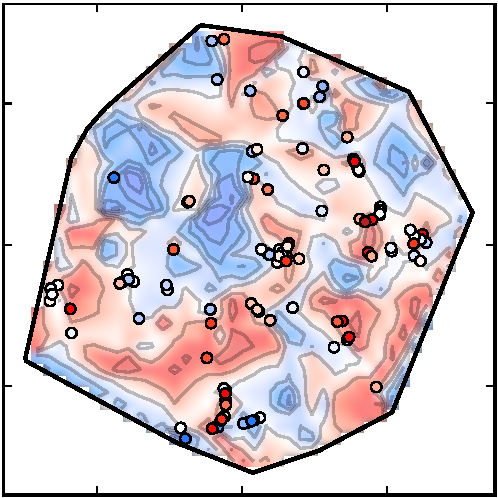
\includegraphics[width= 4.0cm]{neural_networks/images/talk-rac-tsne-t-n}}};}
\visible<9->{\node[anchor=south] (latt) at (5.5,3.15) {{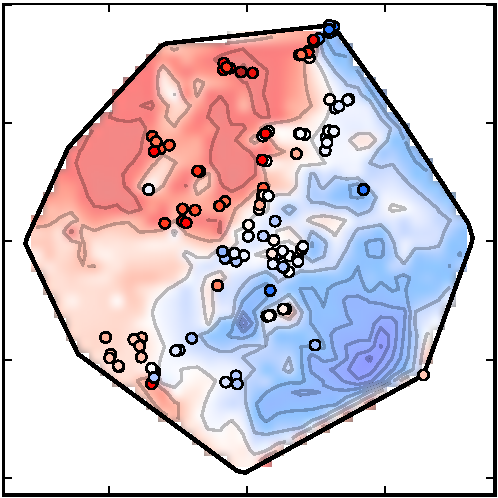
\includegraphics[width= 4.0cm]{neural_networks/images/talk-lat-tsne-t-n}}};}


\def\xof{0.25}
\def\xwd{0.20}
\def\arw{0.10}
\begin{scope}[shift={(0,-0.25)}]
\visible<3->{\draw [black,->,thick, fill=orange] (1.125,3) to [bend left] 
(\xof,3.75) -- (\xof-\arw,3.75) -- (\xof+0.5*\xwd,4.0) -- (\xwd+\xof+\arw,3.75) -- (\xof+\xwd,3.75) to [bend right] (1.125,3.20) --cycle;}
\end{scope}



\def\xof{5.775}
\def\xwd{0.20}
\def\arw{0.10}
\begin{scope}[shift={(0,-0.25)}]
\visible<9->{\draw [black,->,thick, fill=green!50!orange] (4.90,3) to [bend right] 
(\xof+\xwd,3.75)  -- (\xwd+\xof+\arw,3.75)  -- (\xof+0.5*\xwd,4.0) --(\xof-\arw,3.75) -- (\xof,3.75) to [bend left] (4.90,3.20) --cycle;}
\end{scope}
\begin{scope}[shift={(3-1.5*\layersep,-0.5)}]
% draw callout planes
\visible<2->{\node[rectangle, draw, fill=orange, fill opacity=0.15,color=orange, thick,
minimum height = 2.85*\vlayersep cm, minimum width=0.5cm] at (0,3){};}
\visible<8->{\node[rectangle, draw, fill=green!50!orange, fill opacity=0.15,color=green!50!orange, thick,
minimum height = 3.75*\vlayersep cm, minimum width=0.5cm] at (3*\layersep,3){}; }


% Draw the input layer nodes
\foreach \name/\y in {1/3-\vlayersep,2/3,3/3+\vlayersep}{
\visible<2->{\node[input neuron,fill=orange!100 ] (I-\name) at (0,\y) {$ $};}}

% Draw the hidden layer nodes
\foreach \name/\y in {1/3-1.5*\vlayersep,2/3-0.5*\vlayersep,3/3+0.5*\vlayersep,4/3+1.5*\vlayersep}{
	\visible<4->{\path[yshift=0.5] node[hidden neuron] (H-\name) at (\layersep,\y) {\small $ $};}
	\visible<5->{\path[yshift=0.5] node[hidden neuron] (H2-\name) at (2*\layersep,\y) {\small $ $};}
	\visible<6->{\path[yshift=0.5] node[hidden neuron] (H3-\name) at (3*\layersep,\y) {\small $ $};}
}
% Draw the output layer node
\visible<7->{\node[thin, output neuron,pin={[pin edge={->}]right:\footnotesize }] at (3.5*\layersep,3) (O) {$ $};}

\foreach \dest in {1,2,3,4}     
\foreach \source in {1,2,3,4}
{
	\visible<5->{\path[thin,->] (H-\source) edge node[font=\scriptsize] {} (H2-\dest) ;}
	\visible<6->{\path[thin,->] (H2-\source) edge node[font=\scriptsize] {} (H3-\dest) ;}
}

\foreach \source in {1,2,3,4}{
	\visible<7->{\path[thin,->] (H3-\source) edge node[font=\scriptsize] {} (O) ;}}
\foreach \source in {1,2,3}
\foreach \dest in {1,2,3,4}{     
	\visible<4->{\path[thin,->] (I-\source) edge node[font=\scriptsize] {} (H-\dest) ;}}


\visible<2->{
\node[circle, black,thick,minimum width = 2.7cm,minimum height = 2.7cm,path picture={\node at (path picture bounding box.center){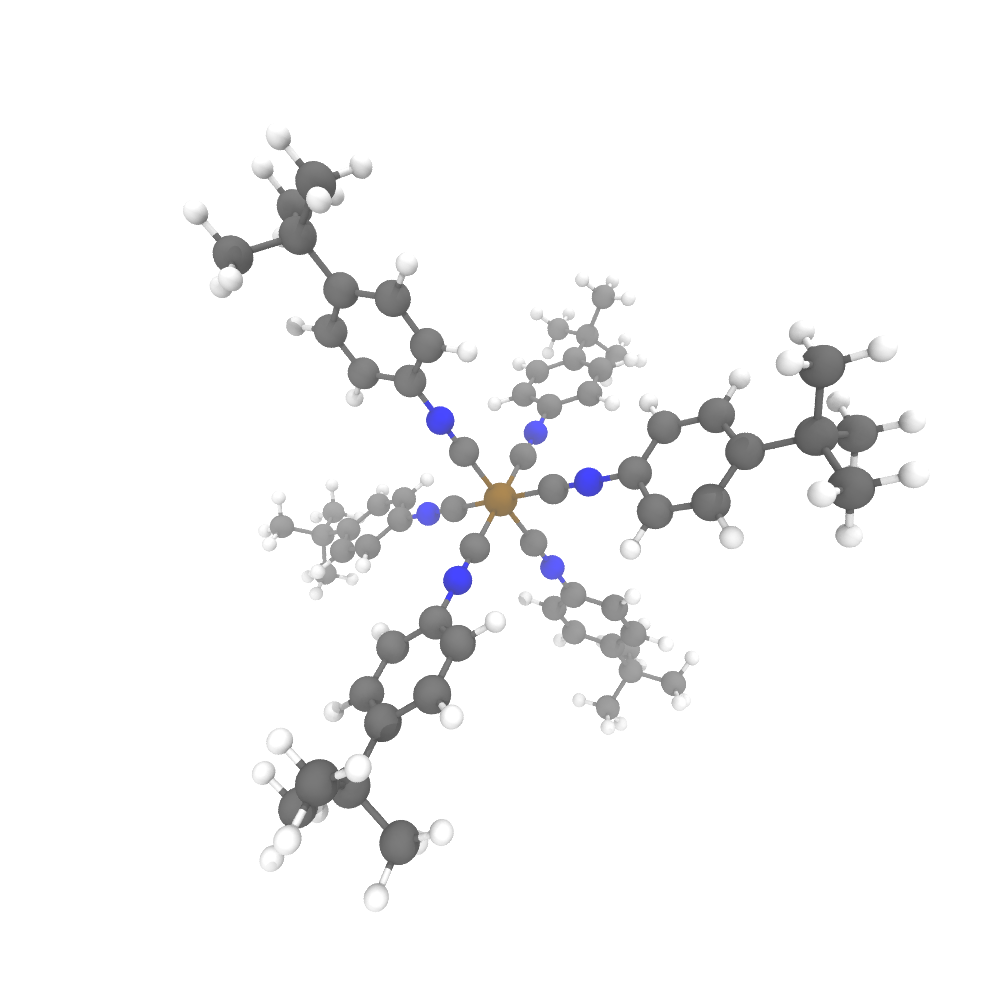
\includegraphics[width=3cm]{representations/images/pisc_trans}}; }] (Xp) at (-2.75,4) {};}

\visible<2->{\node [rotate=0] (ll) at (-1.5,3) {\small input molecule};}
\visible<7->{\node [rotate=0] (l2) at (5.25,3) {\small property};}
\end{scope}	               

%% pane lables
\visible<1->{\node [anchor=south west, text width = 12cm] (la) at (-2.5,7.75) {\small ANNs learn nonlinear reorganizations of the input to make prediciton easier:};}
\visible<3-9>{\node [anchor=south west] (la) at (-1.75,7.25) {\small \textbf{feature space}};}
\visible<9->{\node [anchor=south west] (lb) at (-1.75+5,7.25) {\small \textbf{latent space}};}



\end{tikzpicture}



